\documentclass[12pt]{article}

\usepackage{sbc-template}
\usepackage{graphicx,url}
\usepackage[utf8]{inputenc}
\usepackage[brazil]{babel}
\usepackage{amsmath}

\sloppy

\title{Predição de Acidentes em Rodovias Federais de Santa Catarina por Meio de Aprendizado de Máquina com Atributos Temporais}

\author{Robert Biasoli Drey\inst{1}, Gabrielli Grossi Lara\inst{1}}


\address{Universidade Federal da Fronteira Sul (UFFS)\\
  Campus Chapecó -- Chapecó, SC -- Brasil
}

\begin{document}

\maketitle

\begin{abstract}
This study evaluates monthly crash count forecasts for federal highways in the municipalities of Santa Catarina, Brazil. PRF records from January 2022 to May 2026 were aggregated into municipal monthly series. Four supervised learning algorithms and two baselines were compared using expanding temporal windows. Random Forest with calendar, lagged count and municipality features achieved a mean MAE of 1.76 crashes and WAPE of 32.60\%, reducing mean MAE by 20.7\% relative to the last-month baseline. Errors were larger for higher observed counts. A Streamlit application provides estimates, historical charts and CSV downloads. The findings support the use of historical features within the evaluated scope; operational usefulness and performance after the data cutoff remain untested.

\end{abstract}

\begin{resumo}
Este estudo avalia a previsão mensal da quantidade de sinistros nas rodovias federais dos municípios de Santa Catarina. Os registros da PRF de janeiro de 2022 a maio de 2026 foram agregados por município e mês. Quatro algoritmos supervisionados e dois modelos de referência foram comparados por janelas temporais expansivas. O Random Forest com calendário, defasagens e município obteve MAE médio de 1,76 sinistro e WAPE de 32,60\%, com redução de 20,7\% no MAE médio em relação à repetição do último mês. Os erros foram maiores nas faixas com mais sinistros observados. Uma aplicação Streamlit disponibiliza estimativas, histórico e download em CSV. Os resultados sustentam o uso de atributos históricos no recorte avaliado; a utilidade operacional e o desempenho após o corte da base ainda não foram medidos.

\end{resumo}

\section{Introdução}

As rodovias federais exercem uma função relevante na circulação de pessoas e mercadorias em Santa Catarina, conectando municípios, regiões industriais, áreas de produção agropecuária e acessos portuários. Ao mesmo tempo, os sinistros de trânsito registrados nessas vias provocam mortes, lesões, danos materiais e interrupções no fluxo rodoviário. Em 2014, os sinistros ocorridos nas rodovias federais brasileiras representaram um custo estimado de R\$ 12,3 bilhões para a sociedade \cite{ipea2015acidentes}. Para 2022, uma atualização realizada pela Confederação Nacional do Transporte estimou custos próximos de R\$ 13 bilhões \cite{cnt2023acidentes}. Embora esses valores representem o cenário nacional, eles demonstram a dimensão econômica do problema e complementam seus impactos humanos e sociais.

A distribuição dos sinistros não ocorre de maneira uniforme entre as regiões ou ao longo do tempo. Análises realizadas com dados das rodovias federais brasileiras identificaram variações temporais e regionais no número de vítimas \cite{andrade2019tendencia}. Além disso, fatores como volume de tráfego, características da via, condições meteorológicas e período do ano podem estar associados a diferenças na quantidade de registros. A análise do histórico das ocorrências permite examinar essas variações e identificar tendências e padrões sazonais relevantes para a segurança viária.

A Polícia Rodoviária Federal (PRF) disponibiliza dados abertos sobre os sinistros registrados nas rodovias federais brasileiras, incluindo informações temporais, geográficas e características das ocorrências \cite{prf2026dados}. Esses registros permitem realizar análises descritivas e também construir modelos voltados à previsão da quantidade de sinistros. Entretanto, a previsão exige procedimentos específicos para representar a dependência temporal dos dados e impedir que informações futuras sejam utilizadas durante o treinamento dos modelos.

Técnicas de Aprendizado de Máquina (\textit{Machine Learning} -- ML), por exemplo, já foram utilizadas na identificação de pontos críticos \cite{santos2021machine}, na classificação das causas dos sinistros \cite{rosa2024classificacao} e na predição de sua gravidade \cite{mafort2025tecnicas}. Também existem aplicações de modelos de séries temporais voltadas à previsão de quantidades mensais de sinistros \cite{getahun2021timeseries}. Contudo, essas tarefas diferem quanto à variável prevista, à unidade de análise e ao recorte geográfico adotado.

Neste estudo, o problema foi formulado como uma tarefa de regressão supervisionada com dependência temporal. Os registros individuais da PRF foram agregados por município e mês, e atributos derivados do histórico foram utilizados para estimar a quantidade de sinistros no mês seguinte. A avaliação foi realizada por meio de janelas temporais expansivas, nas quais os modelos são treinados com períodos anteriores e testados em períodos posteriores. Essa organização busca reproduzir as informações que estariam disponíveis no momento de uma previsão e reduzir o risco de vazamento temporal.

A partir dessa delimitação, busca-se responder à seguinte questão de pesquisa: de que forma modelos de Aprendizado de Máquina com atributos temporais podem ser utilizados para prever a frequência mensal de sinistros nas rodovias federais dos municípios de Santa Catarina?

Este artigo tem como objetivo desenvolver e avaliar modelos preditivos para estimar a quantidade de sinistros de trânsito registrada no mês seguinte nas rodovias federais dos municípios de Santa Catarina, utilizando dados abertos da PRF referentes ao período de janeiro de 2022 a maio de 2026.


\section{Fundamentação teórica}

Uma série temporal é composta por observações organizadas segundo sua ordem de ocorrência. Seu comportamento pode apresentar componentes como tendência, sazonalidade e variações irregulares. A tendência representa mudanças de longo prazo, enquanto a sazonalidade corresponde a padrões que se repetem em intervalos regulares \cite{hyndman2021forecasting}.

Problemas de previsão temporal buscam utilizar observações anteriores para estimar valores futuros. Além dos modelos estatísticos específicos para séries temporais, algoritmos de ML podem ser empregados por meio da construção de atributos derivados do histórico. Entre esses atributos estão os valores defasados, as médias móveis e as variáveis de calendário, que permitem representar parte da dependência temporal em um formato adequado a modelos de regressão.

A construção desses atributos deve respeitar o momento em que a previsão é realizada. Para estimar o valor de determinado período, somente podem ser empregadas informações disponíveis até os períodos anteriores. O uso de dados posteriores caracteriza vazamento temporal e pode produzir estimativas excessivamente otimistas sobre o desempenho do modelo.

Para avaliar previsões futuras, a divisão entre treinamento e teste deve reproduzir a disponibilidade das informações no momento da previsão. Neste estudo, foram adotadas janelas expansivas, mantendo o treinamento anterior ao teste, conforme o procedimento de avaliação temporal apresentado por \cite{hyndman2021forecasting}.

Modelos de referência, também denominados \textit{baselines}, são utilizados para determinar um nível básico de desempenho. Uma estratégia simples consiste em repetir o último valor observado, enquanto outra utiliza a média das observações disponíveis no conjunto de treinamento. A comparação com essas abordagens permite verificar se a utilização de modelos mais complexos produz redução efetiva dos erros de previsão \cite{hyndman2021forecasting}.

A avaliação de previsões pode empregar métricas que representam diferentes características dos erros. Medidas como o erro absoluto médio (MAE) e a raiz do erro quadrático médio (RMSE) mantêm relação com a escala da variável prevista, enquanto métricas percentuais permitem interpretar o erro proporcional. Entretanto, métricas baseadas em divisões pelo valor observado exigem cautela quando a série contém valores iguais ou próximos de zero \cite{hyndman2006measures}.

\section{Trabalhos relacionados}

Abordagens de ML foram utilizadas para analisar a distribuição espacial dos sinistros e identificar locais com maior concentração de ocorrências \cite{santos2021machine}. O estudo também analisa a gravidade das ocorrências em Setúbal, Portugal. Sua previsão de pontos críticos difere da estimativa de contagens mensais por município.

No contexto das rodovias brasileiras, técnicas de ML também foram empregadas para classificar as causas de sinistros ocorridos em Minas Gerais \cite{rosa2024classificacao} e para predizer a gravidade de ocorrências registradas em rodovias do Rio de Janeiro \cite{mafort2025tecnicas}. Esses estudos tratam cada sinistro como uma observação e buscam atribuir uma categoria à ocorrência, diferentemente da previsão de uma quantidade mensal agregada.

A evolução temporal das consequências dos sinistros nas rodovias federais brasileiras foi analisada considerando as mudanças no número de vítimas antes e depois da Década de Ação pela Segurança no Trânsito \cite{andrade2019tendencia}. Essa análise demonstra a relevância da dimensão temporal para a compreensão da segurança viária, embora seu objetivo esteja relacionado à identificação de tendências, e não à produção de previsões mensais.

Em uma aplicação diretamente relacionada à previsão de contagens, modelos ARIMA foram utilizados para estimar as quantidades mensais de sinistros, ocorrências fatais e casos com vítimas na região de Amhara, na Etiópia \cite{getahun2021timeseries}. Os registros foram analisados de forma agregada para a região, com dados de quatro zonas da região e sem comparação com os algoritmos de ML avaliados neste projeto.

O Quadro~\ref{tab:comparacao-trabalhos} sintetiza as principais diferenças entre os estudos relacionados e a proposta deste artigo.

\begin{table*}[ht]
\centering
\caption{Comparação entre os trabalhos relacionados e o presente estudo}
\label{tab:comparacao-trabalhos}
\resizebox{\textwidth}{!}{
\begin{tabular}{|p{3.0cm}|p{2.7cm}|p{3.0cm}|p{3.0cm}|p{3.2cm}|}
\hline
\textbf{Estudo} &
\textbf{Problema investigado} &
\textbf{Recorte ou unidade de análise} &
\textbf{Abordagem} &
\textbf{Diferença em relação ao presente estudo} \\
\hline
\cite{santos2021machine} &
Identificação de pontos críticos &
Distrito de Setúbal, Portugal &
Técnicas de ML &
Analisa gravidade e prevê pontos críticos, sem estimar contagens mensais por município. \\
\hline
\cite{rosa2024classificacao} &
Classificação das causas dos sinistros &
Ocorrências em rodovias de Minas Gerais &
Técnicas de ML para classificação &
Prevê categorias associadas às ocorrências individuais, e não quantidades futuras. \\
\hline
\cite{mafort2025tecnicas} &
Predição da gravidade dos sinistros &
Ocorrências em rodovias do Rio de Janeiro &
Técnicas de ML para classificação &
Tem como variável de resposta a gravidade de cada ocorrência. \\
\hline
\cite{andrade2019tendencia} &
Análise de tendências no número de vítimas &
Rodovias federais brasileiras &
Análise temporal &
Analisa tendências históricas, mas não produz previsões mensais por município. \\
\hline
\cite{getahun2021timeseries} &
Previsão da quantidade mensal de sinistros &
Região de Amhara, Etiópia &
Modelos ARIMA &
Realiza previsão regional agregada, sem séries municipais ou comparação com algoritmos de ML. \\
\hline
Presente estudo &
Previsão da quantidade de sinistros no mês seguinte &
Municípios de Santa Catarina com registros em rodovias federais &
Modelos de referência e algoritmos de ML com atributos temporais &
Considera séries mensais por município e emprega validação temporal por janelas expansivas. \\
\hline
\end{tabular}
}
\end{table*}
O presente estudo adota séries mensais por município, enquanto os trabalhos relacionados tratam de classificação, análise espacial ou previsão regional agregada. A comparação com modelos de referência e a validação temporal permitem avaliar essa proposta no recorte catarinense.

\section{Metodologia}

A pesquisa é aplicada e segue a \textit{Design Science Research Methodology} (DSRM), proposta por \cite{peffers2007dsrm}. Suas atividades orientaram a definição do problema, o desenvolvimento, a demonstração, a avaliação e a comunicação do artefato. A seção seguinte relaciona essas entregas às fases do CRISP-ML(Q).

\subsection{Problema e objetivos da solução}

O problema foi delimitado como a previsão da quantidade de sinistros no mês seguinte nas rodovias federais de cada município de Santa Catarina. A solução deveria transformar registros individuais em observações mensais, construir atributos históricos, comparar modelos e disponibilizar as previsões em uma aplicação. Os experimentos deveriam preservar a ordem temporal dos dados e permitir sua reprodução.

\subsection{Coleta e preparação dos dados}

Foram utilizados os microdados abertos da PRF referentes a janeiro de 2022 a maio de 2026 \cite{prf2026dados}. A base filtrada para Santa Catarina reuniu 35.497 ocorrências, distribuídas em 127 municípios e 11 rodovias federais. As datas foram padronizadas e os nomes dos municípios foram convertidos para caixa baixa, com remoção de acentos.

Os registros foram agregados por município e mês, tendo como alvo a quantidade de sinistros (\texttt{qtd\_acidentes}). Para manter séries contínuas, os meses sem registros dentro do período observado receberam valor zero. Foram criadas defasagens de um, dois e doze meses, médias móveis de três e seis meses, acumulado do ano até o mês anterior, média histórica do município e variáveis de calendário. O indicador de alta temporada abrange dezembro, janeiro, fevereiro e julho.

Os atributos históricos utilizam somente meses anteriores ao previsto. Contagens de mortos, feridos e veículos do próprio mês foram excluídas das entradas do modelo implantado, pois não estariam disponíveis no momento da previsão. O município foi codificado por \textit{one-hot}, e o pré-processamento foi ajustado apenas com os dados de treinamento de cada janela.

\subsection{Modelagem e avaliação}

Foram implementados dois modelos de referência: a média do conjunto de treinamento (DummyMedia) e a repetição do último mês (NaiveUltimoMes). Também foram avaliados Regressão Ridge, Regressão de Poisson, Random Forest e HistGradientBoosting. A modelagem utilizou um modelo global para os municípios. Foram comparados calendário; calendário com histórico de sinistros; esses atributos com identificação do município; e a inclusão adicional de histórico de mortos, feridos e veículos. Não foram implementados ARIMA, Prophet ou LSTM. Os experimentos com componentes aleatórios utilizaram semente igual a 42.

Os hiperparâmetros foram definidos manualmente. Ridge utilizou $\alpha=5$ e Poisson, $\alpha=0{,}1$, com até 2.000 iterações. O Random Forest utilizou 250 árvores, no mínimo duas observações por folha e seleção de atributos pela raiz quadrada da quantidade disponível. O HistGradientBoosting utilizou perda quadrática, taxa de aprendizado de 0,06, 300 iterações e regularização $L_2=0{,}1$. As previsões negativas foram limitadas a zero, mantendo valores contínuos para calcular as métricas.

A avaliação empregou quatro janelas expansivas: treinamento em 2022 e teste em 2023; treinamento até 2023 e teste em 2024; treinamento até 2024 e teste em 2025; e treinamento até 2025 e teste de janeiro a maio de 2026. Em cada janela, os modelos foram ajustados novamente com os dados anteriores ao período de teste. O modelo foi reajustado uma vez por janela anual. Dentro do teste, os atributos de cada mês utilizaram as contagens observadas nos meses anteriores, inclusive quando pertenciam ao mesmo ano de teste. Trata-se de previsão de um passo com histórico atualizado, e não de previsão recursiva de todo o ano. As métricas utilizadas estão descritas na seção~\ref{sec:metricas}.

\subsection{Demonstração e comunicação}

O pipeline Random Forest selecionado foi exportado e integrado a uma aplicação Streamlit para consultas por município e mês. O código e as bases processadas foram disponibilizados em repositório público. Este artigo descreve os procedimentos e as limitações do projeto; a implantação do MVP e o plano de manutenção são apresentados a seguir.

\section{Adequação do projeto ao CRISP-ML(Q)}
\label{sec:crispmlq}

O CRISP-ML(Q) organiza o ciclo de vida de aplicações de Aprendizado de Máquina em seis fases, com controles de qualidade em cada etapa \cite{studer2021crispmlq}. Neste projeto, ele complementa a DSRM e relaciona a preparação dos dados e a modelagem das Sprints anteriores ao MVP entregue nesta Sprint.

\subsection{Compreensão do negócio e dos dados}

O projeto busca apoiar o planejamento preventivo da segurança viária por meio da previsão mensal de sinistros nas rodovias federais dos municípios catarinenses. Nas Sprints anteriores, foram definidos a variável-alvo, o recorte de janeiro de 2022 a maio de 2026 e os 127 municípios presentes na base da PRF. A análise exploratória permitiu examinar a distribuição das ocorrências e as diferenças entre municípios.

Os dados representam ocorrências registradas pela PRF, conforme a documentação oficial \cite{prf2026portal}. Por isso, o MVP informa que suas estimativas se referem às rodovias federais, e não a todos os sinistros de cada município. O desempenho técnico é avaliado pelo erro de previsão; a contribuição para decisões de órgãos públicos ainda não foi medida.

\subsection{Preparação dos dados}

Esta fase corresponde aos notebooks de limpeza e construção do \textit{snapshot}, que produziram as bases processadas utilizadas no treinamento e no MVP. Os registros foram filtrados para Santa Catarina, padronizados e agregados por município e mês. A aplicação utiliza essa base para calcular os atributos a partir do município e do mês informados pelo usuário.

O principal controle é o uso exclusivo de dados anteriores ao mês previsto. Também são excluídas as linhas posteriores a maio de 2026 que a grade mensal do \textit{snapshot} preencheu com zero. A aplicação verifica histórico insuficiente, meses ausentes, duplicidades e contagens inválidas. Um teste automatizado compara os atributos da inferência com os utilizados no treinamento.

\subsection{Engenharia de modelagem}

Nas Sprints anteriores, foram comparados modelos de referência e quatro algoritmos supervisionados. O Random Forest com calendário, defasagens e município apresentou o menor MAE médio entre as configurações avaliadas e foi exportado como versão v1. O ajuste final utilizou 6.731 observações mensais, com semente aleatória igual a 42.

O artefato reúne o pré-processamento e o modelo em um pipeline \texttt{joblib}. Seus metadados registram atributos, período de treinamento e métricas. O MVP consome esse artefato e verifica a correspondência entre as entradas e as colunas esperadas. O código, o modelo e as versões das dependências foram registrados no GitHub para permitir a reprodução da aplicação.

\subsection{Avaliação}

A avaliação utilizou janelas temporais expansivas, com testes em 2023, 2024, 2025 e de janeiro a maio de 2026. A versão implantada obteve MAE médio de 1,76 sinistro, RMSE de 2,76 sinistros, WAPE de 32,60\% e $R^2$ de 0,906. São médias dos backtests, calculados com histórico observado anterior a cada mês previsto. As consultas históricas do MVP usam o modelo final, já treinado nesses períodos, e não constituem uma nova avaliação independente.

Cinco testes automatizados, executados novamente em 10 de novembro de 2026, verificaram os atributos, a previsão direta, o tratamento de entradas inválidas, a ausência de vazamento temporal nas entradas e a interação do formulário. Após o deploy, foram conferidos a previsão e o gráfico online. A análise dos erros por município e faixa de contagem foi acrescentada nesta revisão e é apresentada na seção~\ref{sec:resultados}.

\subsection{Implantação}

O MVP foi desenvolvido em Streamlit e publicado no Streamlit Community Cloud em 6 de outubro de 2026. O acesso público está disponível em \url{https://acidentes-sc-pgp.streamlit.app/}. O usuário seleciona município e mês e recebe a estimativa, o gráfico do histórico e a opção de baixar o resultado em CSV. A interface também apresenta a versão do modelo e suas métricas de validação.

A aplicação utiliza Python 3.12, o modelo v1 e os dados versionados no repositório \url{https://github.com/dreyrobert/pgp_machine_learning}, que contém as instruções de uso e deploy. Como a base termina em maio de 2026, a previsão futura disponível é junho de 2026. Os controles incluem dependências fixadas, cache de carregamento e mensagens para falhas na leitura dos arquivos. Nesta revisão, foram acrescentadas ao MVP a comparação com a repetição do último mês e a consulta aos erros dos backtests por município e faixa de contagem. A atualização online desses recursos depende da publicação do código na branch de deploy.

\subsection{Monitoramento e manutenção}

O CRISP-ML(Q) inclui o acompanhamento do modelo após a implantação \cite{studer2021crispmlq}. Atualmente, o projeto mantém metadados, testes e histórico de commits, mas ainda não possui detecção automática de \textit{drift}, alertas ou retreinamento agendado. Essa etapa permanece como trabalho futuro.

A proposta é incorporar cada novo mês completo da PRF, verificar a qualidade dos dados e comparar previsões previamente registradas com os valores observados. MAE, RMSE e WAPE deverão ser acompanhados por período e município, incluindo a comparação com a repetição do último mês. Alterações persistentes no desempenho deverão motivar a revisão dos dados e a avaliação de uma nova versão por validação temporal. Os critérios de alerta ainda precisam ser definidos. A versão anterior deverá ser preservada para permitir retorno em caso de falhas, considerando os riscos de manutenção associados a dados e configurações de sistemas de ML \cite{sculley2015debt}.

\section{Métricas de avaliação}
\label{sec:metricas}

Os modelos foram comparados por MAE, RMSE, MAPE, WAPE e $R^2$ \cite{hyndman2006measures}. As métricas foram calculadas em cada janela temporal e resumidas pela média dos quatro períodos de teste.

O MAE expressa o erro médio em número de sinistros. O RMSE mantém essa unidade, mas atribui maior peso aos erros elevados. Ambas as medidas devem ser minimizadas.

O MAPE foi calculado somente para observações com pelo menos um sinistro, pois envolve divisão pelo valor observado. Como contagens baixas podem gerar percentuais elevados mesmo com pequenos erros absolutos, essa métrica foi utilizada como medida complementar. O WAPE relaciona a soma dos erros absolutos ao total de sinistros e inclui meses com contagem zero, desde que o total do período seja positivo.

O $R^2$ compara os erros do modelo à variação dos valores observados em torno de sua média. Valores próximos de um indicam melhor ajuste; valores negativos indicam desempenho inferior à previsão pela média do conjunto avaliado.

A comparação priorizou menores valores de MAE e WAPE, pela interpretação do erro absoluto e pela presença de meses sem registros. RMSE, MAPE e $R^2$ complementaram a análise.



\section{Resultados}
\label{sec:resultados}

A Tabela~\ref{tab:modelos} compara os modelos nas quatro janelas de teste. Para os algoritmos supervisionados, são apresentados os resultados com calendário, histórico de sinistros e município, conjunto utilizado no MVP. Os valores são médias simples das métricas de cada janela; assim, janeiro a maio de 2026 recebe o mesmo peso que cada ano completo.

\begin{table}[ht]
\centering
\caption{Médias dos backtests temporais. MAE e RMSE em sinistros por município-mês.}
\label{tab:modelos}
\begin{tabular}{lrrrr}
\hline
Modelo & MAE & RMSE & WAPE (\%) & $R^2$ \\
\hline
Random Forest & 1,756 & 2,764 & 32,60 & 0,906 \\
Ridge & 1,798 & 2,816 & 33,45 & 0,902 \\
HistGradientBoosting & 1,897 & 3,046 & 35,25 & 0,885 \\
Repetição do último mês & 2,215 & 3,535 & 41,07 & 0,845 \\
Poisson & 2,484 & 4,148 & 46,11 & 0,785 \\
Média do treinamento & 5,128 & 9,013 & 95,18 & -0,001 \\
\hline
\end{tabular}
\end{table}

O Random Forest com esses atributos apresentou o menor MAE médio entre todas as configurações avaliadas. A redução foi de 20,7\% em relação à repetição do último mês, calculada pela diferença entre os MAEs médios dividida pelo MAE médio da referência. Em relação ao Ridge, a redução foi de 2,3\%. O conjunto com histórico adicional de severidade e veículos obteve RMSE ligeiramente menor, de 2,750, mas MAE maior, de 1,764. A escolha do modelo priorizou o MAE.

\begin{table}[ht]
\centering
\caption{Random Forest implantado: desempenho por janela de teste.}
\label{tab:anos}
\begin{tabular}{lrrrrr}
\hline
Teste & Observações & MAE & RMSE & WAPE (\%) & $R^2$ \\
\hline
2023 & 1.524 & 1,732 & 2,612 & 33,85 & 0,908 \\
2024 & 1.524 & 1,710 & 2,667 & 31,10 & 0,916 \\
2025 & 1.524 & 1,733 & 2,761 & 32,27 & 0,905 \\
Jan.--maio/2026 & 635 & 1,850 & 3,017 & 33,20 & 0,894 \\
\hline
\end{tabular}
\end{table}

O MAE variou de 1,710 em 2024 a 1,850 em 2026. O último período teve o maior MAE e RMSE, mas corresponde a apenas cinco meses e não permite concluir que exista uma tendência de degradação.

\subsection{Erros por município e quantidade observada}

As 5.207 previsões de teste foram reunidas para examinar os erros por faixa de contagem (Tabela~\ref{tab:faixas}). Essas métricas foram calculadas diretamente sobre as previsões agrupadas, sem a média por janela. O viés corresponde à média de previsto menos observado: valores negativos indicam subestimação.

\begin{table}[ht]
\centering
\caption{Erros do Random Forest por quantidade observada no município-mês.}
\label{tab:faixas}
\begin{tabular}{lrrrr}
\hline
Sinistros observados & Observações & MAE & WAPE (\%) & Viés \\
\hline
0 & 1.115 & 0,934 & --- & 0,934 \\
1--5 & 2.723 & 1,230 & 48,22 & 0,411 \\
6--10 & 705 & 2,351 & 30,79 & -0,922 \\
11--20 & 367 & 3,856 & 27,56 & -1,207 \\
21 ou mais & 297 & 5,386 & 15,32 & -2,503 \\
\hline
\end{tabular}
\end{table}

O erro absoluto aumenta nas faixas de maior contagem, enquanto o WAPE diminui. Nos meses sem sinistros, o modelo estimou em média 0,934 ocorrência; o WAPE não é definido nessa faixa porque o total observado é zero. Para 21 ou mais sinistros, houve subestimação média de 2,503 ocorrências. As faixas foram definidas pelo valor observado após o teste e servem à análise dos erros, sem representar categorias conhecidas antecipadamente pelo modelo.

Na análise municipal, São José apresentou o maior MAE, de 8,829 sinistros, seguido por Palhoça, com 6,309, e Araquari, com 5,875. Os WAPEs foram, respectivamente, 14,17\%, 13,02\% e 23,12\%. A diferença entre essas medidas mostra que um erro absoluto maior pode representar uma parcela menor do volume observado. A Figura~\ref{fig:backtest} apresenta os três municípios com maior total observado no teste, escolhidos pelo volume, sem seleção pelo ajuste do modelo.

\begin{figure}[ht]
\centering
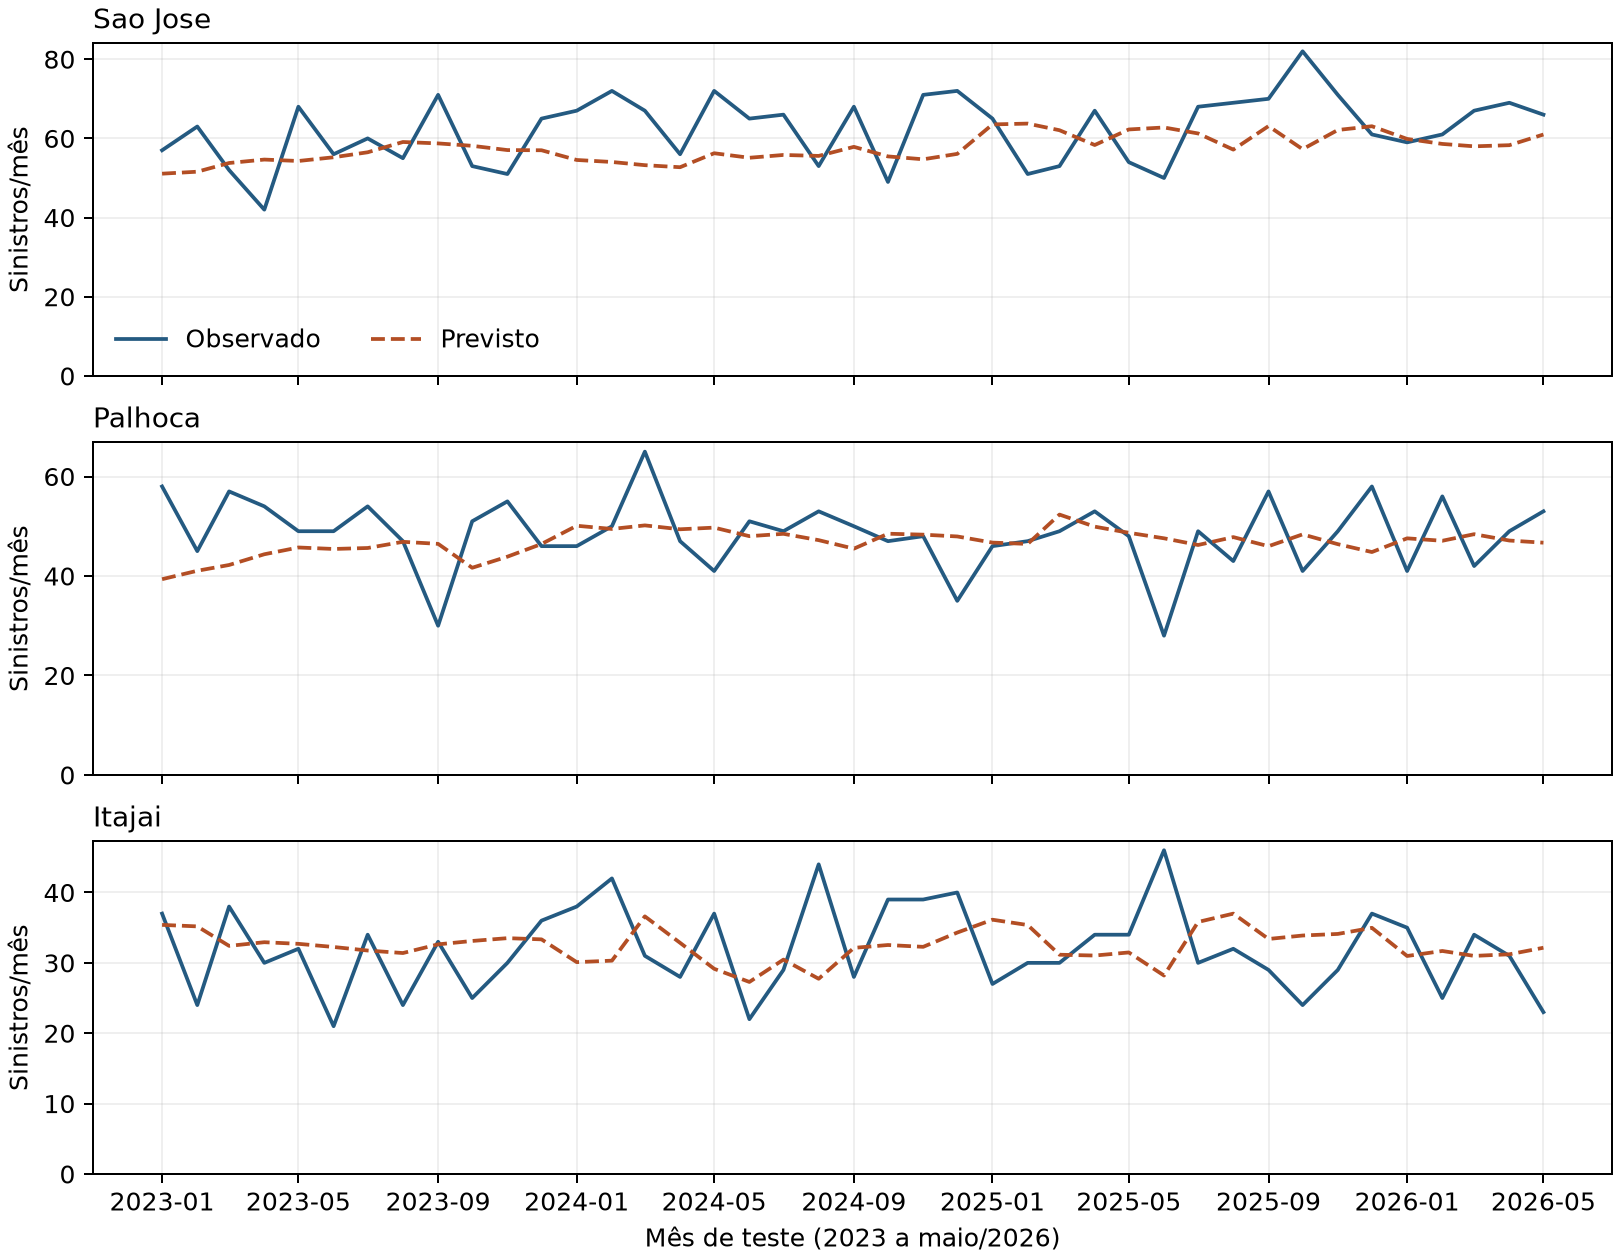
\includegraphics[width=0.9\textwidth]{../docs/graphics/backtest_rf_municipios.png}
\caption{Valores observados e previsões dos backtests nos três municípios com maior total de sinistros no teste.}
\label{fig:backtest}
\end{figure}

\section{Discussão}

A comparação com a repetição do último mês indica que os atributos históricos, combinados ao Random Forest, reduziram o erro no recorte avaliado. Usando apenas calendário, o Random Forest teve MAE médio de 5,223; ao acrescentar o histórico de sinistros, o valor caiu para 1,770. A inclusão do município reduziu o MAE para 1,756. O principal ganho observado ocorreu, portanto, com a inclusão do histórico, enquanto a identificação do município trouxe uma redução menor.

A importância de permutação calculada no teste de janeiro a maio de 2026 também destacou o histórico. Embaralhar a média histórica municipal aumentou o MAE em 0,833 sinistro, em média; para a média móvel de seis meses, o aumento foi de 0,557. Esses valores medem a dependência preditiva do modelo em relação aos atributos e não demonstram causas dos sinistros. A correlação entre atributos históricos também limita sua interpretação isolada.

O $R^2$ médio de 0,906 deve ser interpretado junto aos erros absolutos e percentuais. Ele foi calculado sobre municípios com volumes diferentes e não demonstra que o modelo acompanha igualmente bem as oscilações de cada série municipal. A superestimação nas contagens baixas e a subestimação nas altas reforçam essa restrição. O cuidado com métricas percentuais em séries com zeros e valores baixos é discutido por \cite{hyndman2006measures}.

O trabalho de \cite{getahun2021timeseries} também utiliza contagens mensais, mas adota modelos ARIMA em outro recorte geográfico. Já \cite{rosa2024classificacao} e \cite{mafort2025tecnicas} investigam categorias de ocorrências individuais. Por essas diferenças de alvo, dados e validação, seus resultados não permitem estabelecer superioridade numérica do modelo deste projeto.

O MVP permite consultar e exportar estimativas, mas sua contribuição ao planejamento preventivo ainda precisa ser avaliada com usuários. Os erros podem orientar a leitura das previsões, sobretudo nos municípios de maior volume. Entretanto, o estudo não mediu mudanças na alocação de recursos nem redução de sinistros após o uso da aplicação.

\section{Limitações}

A base contém registros da PRF em rodovias federais de Santa Catarina. As previsões não abrangem todas as vias dos municípios nem permitem generalização direta para outros estados. A ausência de registro em um mês foi tratada como zero dentro do período coberto pelos arquivos; isso não comprova a ausência de ocorrências não registradas. O escopo dos registros deve ser interpretado conforme a documentação da PRF \cite{prf2026portal}.

O modelo estima contagens, sem medidas de exposição, como fluxo de veículos ou distância percorrida. Assim, uma quantidade maior de sinistros não equivale necessariamente a maior risco por veículo. Também não foram incorporadas medidas externas de clima, intervenções viárias ou mudanças de tráfego.

A seleção do modelo e a comparação dos atributos utilizaram as mesmas quatro janelas. Não foi reservado um período adicional, intocado durante essa seleção, e não foram realizados testes de significância ou intervalos de confiança para as diferenças entre modelos. O pequeno ganho sobre o Ridge não permite afirmar superioridade estatística. Os hiperparâmetros foram definidos manualmente, e a comparação não inclui modelos específicos de séries temporais.

Os backtests utilizam valores observados dos meses anteriores e pressupõem sua disponibilidade antes de cada previsão. Não foi avaliado o atraso de publicação dos dados da PRF. Os resultados também não representam previsões recursivas para vários meses. O preenchimento inicial de atributos históricos ausentes com zero é outra simplificação.

A base termina em maio de 2026 e o MVP permite somente junho de 2026 como passo futuro. Não há avaliação posterior ao corte, intervalos de previsão ou validação com usuários. As consultas históricas do MVP usam o modelo final treinado nesses períodos e não substituem os backtests. Monitoramento automático e retreinamento ainda não foram implementados, atividades relevantes à manutenção de sistemas de ML \cite{sculley2015debt}.

\section{Conclusão}

Os experimentos mostram que modelos supervisionados com atributos do histórico podem estimar contagens mensais de sinistros no recorte estudado. O Random Forest apresentou o menor MAE médio e reduziu essa medida em 20,7\% em relação à repetição do último mês. A análise por faixas revelou superestimação nas contagens baixas e subestimação nas altas, o que limita o uso de uma única métrica agregada para avaliar a solução.

O projeto entrega preparação de dados, comparação temporal de modelos e um MVP para consulta das estimativas. Os próximos passos são atualizar o histórico, avaliar uma nova janela sem utilizá-la na seleção do modelo e testar a aplicação com usuários. Esses procedimentos são necessários para avaliar sua utilidade operacional.

\bibliographystyle{sbc}
\bibliography{referencias,crisp-ml-references}

\end{document}
